\documentclass[dynamic_systems.tex]{subfiles}
\begin{document}

\chapter[Transient response]{Qualities of transient response}
\tags{}

In this chapter, we explore the qualities of transient response---the response of the system in the interval during which initial conditions dominate.
\tags{}

We focus on characterizing first- and second-order linear systems; not because they're easiest (they are), but because nonlinear systems can be \keyword[linearization]{linearized} about an \keyword{operating point} and because higher-order linear system responses are just \emph{sums of first- and second-order responses}, making ``everything look first- and second-order.''
Well, many things, at least.
\tags{}

In this chapter, we primarily consider systems represented by \keyword[SISO]{single-input, single-output (SISO)} ordinary differential equations (also called io ODEs)---with variable $y$ representing the \emph{output}, dependent variable time $t$, variable $u$ representing the \emph{input}, \keyword{forcing function} $f$, constant coefficients $a_i,b_j$, order $n$, and $m \le n$ for $n\in\mathbb{N}_0$---of the form
\tags{}

\begin{subequations}
\begin{alignat}{8}
\label{eq:ioode1}
	\dfrac{d^n y}{d t^n} & {}+{} & 
	a_{n-1} \dfrac{d^{n-1} y}{d t^{n-1}} & {}+{} & 
	\cdots  & {}+{} &
	a_1 \dfrac{d y}{d t}  & {}+{} && 
	a_0 y = f \text{, where} \\
	f \equiv b_m \dfrac{d^m u}{d t^m}  & {}+{} & 
	b_{m-1} \dfrac{d^{m-1} u}{d t^{m-1}}  & {}+{} & 
	\cdots & {}+{} & 
	b_1 \dfrac{d u}{d t} & {}+{} &&
	b_0 u. \label{eq:ioode2}
\end{alignat}
\end{subequations}

Note that the forcing function $f$ is related to but distinct from the input $u$.
This terminology proves rather important.
\tags{}

\section{Characteristic transient responses}
\tags{}

A system's \keyword[characteristic response]{characteristic responses} are responses to specific forcing functions---called the \keyword{singularity functions}.
The reasons these are ``characteristic'' are:
\tags{}
\begin{enumerate}
	\item the singularity functions model commonly interesting system inputs (e.g.\ a sudden change in the input), and so they can be said to \emph{characterize inputs}, and
	\item the ways in which the system responds to these specific functions reveal aspects of the system (e.g.\ how quickly it responds), so these responses can be said to \emph{characterize systems}.
\end{enumerate}

Now, one may object that \autoref{eq:ioode2} shows that a forcing function needn't look anything like an input due to its being composed of a sum of scaled copies of the input and its derivatives.
Yes, but given two key properties of linear, time-invariant (LTI) systems---\keyword{superposition} and the \keyword{differentiation} property---, knowing a system's response $y_1$ to a forcing function $f_1$ allows us to construct its response to that input (that is, $y_2$ for input $u_2 = f_1$) as
\tags{}
\maybeeq{%
\begin{align*}
y_2 = 
b_m \dfrac{d^m y_1}{d t^m} {}+{} 
	b_{m-1} \dfrac{d^{m-1} y_1}{d t^{m-1}}  {}+{} 
	\cdots & {}+{} 
	b_1 \dfrac{d y_1}{d t} {}+{}
	b_0 y_1.
\end{align*}%
}
\noindent I \href{http://ricopic.one/resources/mind_blown.gif}{know}.

There are three singularity functions, which are now defined as piecewise functions of time $t$.
\tags{}

First, the \keyword{unit impulse} or \keyword{Dirac delta} function\footnote{Technically, $\delta$ is a distribution, not a function, but we use the common, confusing, comfortably couched terminology.} $\delta$ is defined as zero everywhere except at $t=0$, when it is undefined, and has unity as its integral over all time.
When $\delta$ is scaled (e.g. $5\delta$), its integral scales by the same factor.
This strange little beast models a sudden ``spike'' in the input.
\tags{}

Second, the \keyword{unit step} function $u_s$ is defined as zero for $t \le 0$ and unity for $t>0$.
It models a sudden change in the input.
Scaling it scales the amount of change.
Often, this is considered to be the gold-standard for characterizing the transient response of a system.%, so we pay it special attention in the following lectures.
\tags{}

Third, the \keyword{unit ramp} function $u_r$ is defined as zero for $t \le 0$ and $t$ for $t>0$---that is, it is linearly increasing with unity slope.
It models a steadily increasing input and is probably the least useful of the singularity functions.
Scaling it scales the rate of steady change.
\tags{}

\section[First-order systems]{First-order systems in transient response}
\tags{}

First order systems have input-output differential equations of the form
\begin{align}
	\label{eq:io_ode_first_order}
	\tau \dfrac{d y}{d t} + y = b_1 \dfrac{d u}{d t} + b_0 u
\end{align}

with $\tau\in\mathbb{R}$ called the \keyword{time constant} of the system.
Systems with a single energy storage element---such as those with electrical or thermal capacitance---can be modeled as first-order.
\tags{C}

The characteristic equation yields a single root $\lambda = -1/\tau$, so the \keyword{homogeneous solution} $y_h$, for constant $\kappa\in\mathbb{R}$, is
\maybeeq{%
\begin{align*}
	y_h(t) = \kappa\,e^{-t/\tau}.
\end{align*}%
}

\subsection{Free response}
\tags{}

The \keyword{free response $y_\textnormal{fr}$} of a system is its response to initial conditions and no forcing ($f(t) = 0$).
This is useful for two reasons:
\tags{}
\begin{enumerate}
	\item perturbations of the system from equilibrium result in free response and
	\item from superposition, the free response can be added to a forced response to find the specific response: $y(t) = y_\text{fr}(t) + y_\text{fo}(t)$. This allows us to use tables of solutions like \autoref{tab:forced_response_first_order} to construct solutions for systems with nonzero initial conditions with forcing.
\end{enumerate}

The free response is found by applying initial conditions to the homogeneous solution. 
With initial condition $y(0)$, the free response is
\tags{}
\begin{align}\label{eq:free1}
	y_\text{fr}(t) = y(0)\, e^{-t/\tau},
\end{align}
which begins at $y(0)$ and decays exponentially to zero.

\subsection{Step response}
\tags{}

In what follows, we develop \keyword{forced response $y_\textnormal{fo}$} solutions, which are the \emph{specific solution} responses of systems to given inputs and \keyword{zero initial conditions}: all initial conditions set to zero.
\tags{}

If we consider the common situation that $b_1 = 0$ and $u(t) = K u_s(t)$ for some $K\in\mathbb{R}$, the solution to \autoref{eq:io_ode_first_order} is
\maybeeq{
	\begin{align*}
		y_\text{fo}(t) &= K b_0 (1 - e^{-t/\tau}).
	\end{align*}
}
\noindent The non-steady term is simply a constant scaling of a decaying exponential.

\begin{figure}[b]
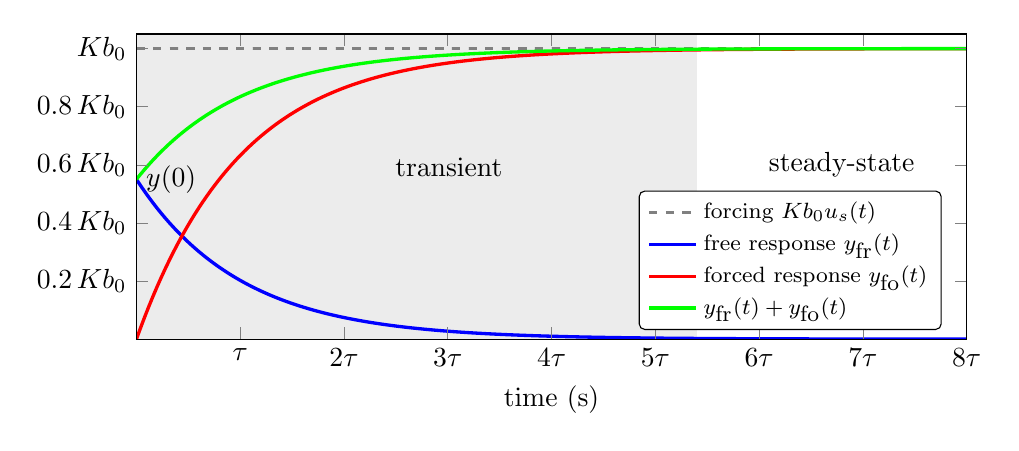
\begin{tikzpicture}
\newcommand{\taunow}{1.0}
\newcommand{\ynot}{0.55}
\newcommand{\yss}{1.0}
\begin{axis}[
xlabel={time (s)},
xmin=0, xmax=8,
ymin=0, ymax=1.05,
axis on top,
width=1\linewidth,
height=.45\linewidth,
xtick={1,2,3,4,5,6,7,8},
xticklabels={$\tau$,$2\tau$,$3\tau$,$4\tau$,$5\tau$,$6\tau$,$7\tau$,$8\tau$},
ytick={.2,.4,.6,.8,1},
yticklabels={$0.2\,K b_0$,$0.4\,K b_0$,$0.6\,K b_0$,$0.8\,K b_0$,$K b_0$},
tick pos=both,
tick label style={/pgf/number format/fixed},
scaled ticks=false,
legend entries={{forcing $K b_0 u_s(t)$},{free response $y_\textnormal{fr}(t)$},{forced response $y_\textnormal{fo}(t)$},{$y_\textnormal{fr}(t) + y_\textnormal{fo}(t)$}},
legend style={
	legend pos=south east,
	cells={anchor=west},
	font=\footnotesize,
	rounded corners=2pt,
}
]

\fill [gray!15] (rel axis cs:0,0) rectangle (rel axis cs:.675,1);
\node at (rel axis cs:.3,.5) [anchor=south west] {transient};
\node at (rel axis cs:.75,.5) [anchor=south west] {steady-state};
\addplot[
gray,
dashed,
very thick,
domain=0:8,
samples=201,
] {1};
\addplot[
blue,
very thick,
domain=0:8,
samples=201,
] {(\ynot)*e^(-x/\taunow)};
\addplot[
red,
very thick,
domain=0:8,
samples=201,
] {(-\yss)*e^(-x/\taunow) + \yss};
\addplot[
green,
very thick,
domain=0:8,
samples=201,
] {(\ynot-\yss)*e^(-x/\taunow) + \yss};
\node at (axis cs:0,\ynot) [anchor=west] {$y(0)$};
\end{axis}
\end{tikzpicture}
\caption{free and forced responses and their sum for a first order system with input $u(t) = K u_s(t)$, initial condition $y(0)$, and $b_1=0$.}
\label{fig:first_order_step_response}
\end{figure}

A plot of the step response is shown in \autoref{fig:first_order_step_response}.
As with the free response, within $5\tau$ the transient response is less than $1\%$ of the difference between $y(0)$ and steady-state.
\tags{}

\subsection{Impulse and ramp responses}
\tags{}

The response to all three singularity inputs are included in \autoref{tab:forced_response_first_order}.
These can be combined with the free response of \autoref{eq:free1} using superposition.
Results could be described as \keyword[bitchin']{\href{http://ricopic.one/resources/bitchin.gif}{bitchin'}}.
\tags{}

\begin{table}
\centering
\caption{first-order system characteristic and total forced responses for singularity inputs. The relevant differential equation is of the standard form $\tau \dot{y} + y = f$.}
\begin{tabular}{m{.07\columnwidth} m{.32\columnwidth} m{.47\columnwidth}}
	\toprule
	$u(t)$		& characteristic response		& total forced response $y_\text{fo}$ for $t \ge 0$ \\
	 & $f(t) = u(t)$ & $f(t) = b_1 \dot{u} + b_0 u$ \\ \midrule
	${\delta}(t)$	& $\dfrac{1}{\tau} e^{-t/\tau}$			& $\dfrac{b_1}{\tau} \delta(t) + \left (\dfrac{b_0}{\tau} - \dfrac{b_1}{\tau^2} \right ) e^{-t/\tau}$ \\
	$u_s(t)$		& $1 - e^{-t/\tau}$					& $b_0 - \left ( b_0 - \dfrac{b_1}{\tau} \right ) e^{-t/\tau}$ \\
	$u_r(t)$		& $t - \tau (1-e^{-t/\tau})$				& $b_0 t + (b_1 - b_0 \tau)(1-e^{-t/\tau})$ \\
	\bottomrule
\end{tabular}
\label{tab:forced_response_first_order}
\end{table}

\examplemaybe{
 	RC-circuit response the easy way
}{
	Consider a parallel RC-circuit with input current $I_S(t) = 2 u_s(t)$ A, initial capacitor voltage $v_C(0) = 3$ V, resistance $R = 1000\ \Omega$, and capacitance $C = 1$ mF. Proceeding with the usual analysis would produce the io differential equation
	\begin{align*}
	C \frac{d v_C}{d t} + v_C/R = I_S.
	\end{align*}
	Use \cref{tab:forced_response_first_order} to find $v_C(t)$.
}{
  \begin{enumerate}
  	\item
  	First, we recognize that the input is $u = I_S$ and the output is $y = v_C$.
  	\item 
	  Rewrite the differential equation in standard form:
	  \begin{align*}
	  	R C \frac{d v_C}{d t} + v_C = R I_S.
	  \end{align*}
	  From inspection:
	  \begin{align*}
	  	\tau = R C 
	  	\quad \text{and} \quad
	  	f(t) = R I_S(t) = 2 R u_s(t).
	  \end{align*}
	  \item 
	  We choose to use superposition and \cref{tab:forced_response_first_order}.
	  From \cref{eq:free1}, the free response is
	  \begin{align*}
	  	y_\textnormal{fr}(t) = v_C(0) e^{-t/\tau} = 3 e^{-t/\tau}.
	  \end{align*}
	  From \cref{tab:forced_response_first_order}, the characteristic response for $f(t) = u_s(t)$ is
	  \begin{align*}
	  	y_\textnormal{ch}(t) = 1 - e^{-t/\tau}.
	  \end{align*}
	  Since our $f(t) = 2 R u_s(t)$, the forced response is
	  \begin{align*}
	  	y_\textnormal{fo}(t) = 2 R y_\textnormal{ch}(t) =  2 R (1 - e^{-t/\tau}).
	  \end{align*}
	  Finally, the specific solution for $y(t) = v_C(t)$ is 
	  \begin{align*}
	  	y(t) &= y_\textnormal{fr}(t) + y_\textnormal{fo}(t) \\
	  	&= 3 e^{-t/\tau} + 2 R (1 - e^{-t/\tau}) \\
	  	&= 2 R + (3 - 2 R) e^{-t/\tau}.
	  \end{align*}
	  % \vspace{10\baselineskip}
  \end{enumerate}
}{%
ex:response_first_order%
}

\section[Second-order systems]{Second-order systems in transient response}
\tags{}

Second-order systems have input-output differential equations of the form
\begin{equation}\label{eq:ioode_second_order}
	\dfrac{d^2 y}{dt^2} + 2 \zeta \omega_n \dfrac{dy}{dt} + \omega_n^2 y = f(t)
\end{equation}
where $\omega_n$ is called the \keyword[natural frequency $\omega_n$]{natural frequency}, $\zeta$ is called the (dimensionless) \keyword[damping ratio $\zeta$]{damping ratio}, and $f$ is a forcing function that depends on the input $u$ as
\begin{align}
	f(t) = b_2\dfrac{d^2 u}{d t^2} + b_1\dfrac{d u}{d t} + b_0 u.
\end{align}
Systems with two energy storage elements---such as those with an inertial element and a spring-like element---can be modeled as second-order.
\tags{}

For distinct roots ($\lambda_1\ne\lambda_2$), the homogeneous solution is, for some real constants $\kappa_1$ and $\kappa_2$,
\begin{equation} \label{eq:homo2}
	y_h(t) = \kappa_1 e^{\lambda_1 t} + \kappa_2 e^{\lambda_2 t}
\end{equation}
where
\begin{equation} \label{eq:lambda2}
	\lambda_1 \text{, } \lambda_2 = -\zeta \omega_n \pm \omega_n \sqrt{\zeta^2 - 1}.
\end{equation}

\subsection{Free response}
\tags{}
\label{lec:second_order_free_response}

The free response $y_\textnormal{fr}$ is found by applying initial conditions to the homogeneous solution. 
With initial conditions $y(0)$ and $\dot{y}(0) = 0$, the free response is
\tags{}
\begin{align}\label{eq:homo3}
	y_\text{fr}(t) = y(0) \dfrac{1}{\lambda_2-\lambda_1} 
	\left(
		\lambda_2 e^{\lambda_1 t} -
		\lambda_1 e^{\lambda_2 t}
	\right).
\end{align}
There are five possibilities for the location of the roots $\lambda_1$ and $\lambda_2$, all determined by the value of $\zeta$.
\begin{description}
	\item[$\zeta \in (-\infty,0)$: unstable]
		This case is very undesirable because it means our system is unstable and, given any nonzero input or output, will \keyword[boom \Xey]{explode \Xey} to infinity.
	\item[$\zeta = 0$: undamped]
		An undamped system will oscillate forever if perturbed from zero output.
	\item[$\zeta \in (0,1)$: underdamped]
		Roughly speaking, underdamped systems oscillate, but not forever.
		Let's consider the form of the solution for initial conditions and no forcing. 
		The roots of the characteristic equation are
		\begin{equation}
			\lambda_1 \text{, } \lambda_2 = -\zeta \omega_n \pm j \omega_n \sqrt{1 - \zeta^2} = -\zeta \omega_n \pm j \omega_d
		\end{equation}
		where the \keyword{damped natural frequency $\omega_d$} is defined as
		\begin{equation}
			\omega_d \equiv \omega_n \sqrt{1-\zeta^2}.
		\end{equation}
		From Equation~\eqref{eq:homo3} for the free response, using Euler's formulas to write in terms of trigonometric functions, and the initial conditions $y(0)$ and $\dot{y}(0) = 0$, we have
		\begin{align}\label{eq:underdamped_response}
			y_\text{fr}(t) = y(0) \dfrac{e^{-\zeta \omega_n t}}{\sqrt{1-\zeta^2}} \cos (\omega_d t + \psi)
		\end{align}
		where the phase $\psi$ is
		\begin{equation}
			\psi =  -\arctan\dfrac{\zeta}{\sqrt{1-\zeta^2}}.
		\end{equation}
		This is an oscillation that decays to the value it oscillates about, $y(t)|_{t\rightarrow\infty}=0$.
		So any perturbation of an underdamped system will result in a decaying oscillation about equilibrium.
	\item[$\zeta = 1$: critically damped]
		In this case, the roots of the characteristic equation are equal:
		\begin{equation}
			\lambda_1 = \lambda_2 = -\omega_n
		\end{equation}
		So we must modify \autoref{eq:homo2} with a factor of $t$ for the homogeneous solution.
		The free response for initial conditions $y(0)$ and $\dot{y}(0) = 0$, we have
		\begin{align}
			y_\text{fr}(t) = y(0) \left ( 1 + \omega_n t \right ) e^{-\omega_n t}.
		\end{align}
		This decays without oscillation, but just barely.
	\item[$\zeta \in (1,\infty)$: overdamped]
		Here the roots of the characteristic equation are distinct and real.
		From Equation~\eqref{eq:homo3} with free response to initial conditions $y(0)$ and $\dot{y}(0) = 0$, we have the sum of two decaying real exponentials.
		This response will neither overshoot nor oscillate---like the critically damped case---but with even less gusto.
\end{description}

\autoref{fig:second_order_free_response} displays the free response results.
Note that a small damping ratio results in overshooting and oscillation about the equilibrium value.
In contrast, large damping ratio results in neither overshoot nor oscillation.
However, both small and large damping ratios yield responses that take longer durations to approach equilibrium than damping ratios near unity.
% For this reason, the damping ratio of a system should be close to one.
In terms of system performances, there are tradeoffs on either side of $\zeta=1$.
Slightly less than one yields faster responses that overshoot a small amount.
Slightly greater than one yields slower responses less prone to oscillation.
\tags{B, D}

\begin{figure}[bt]
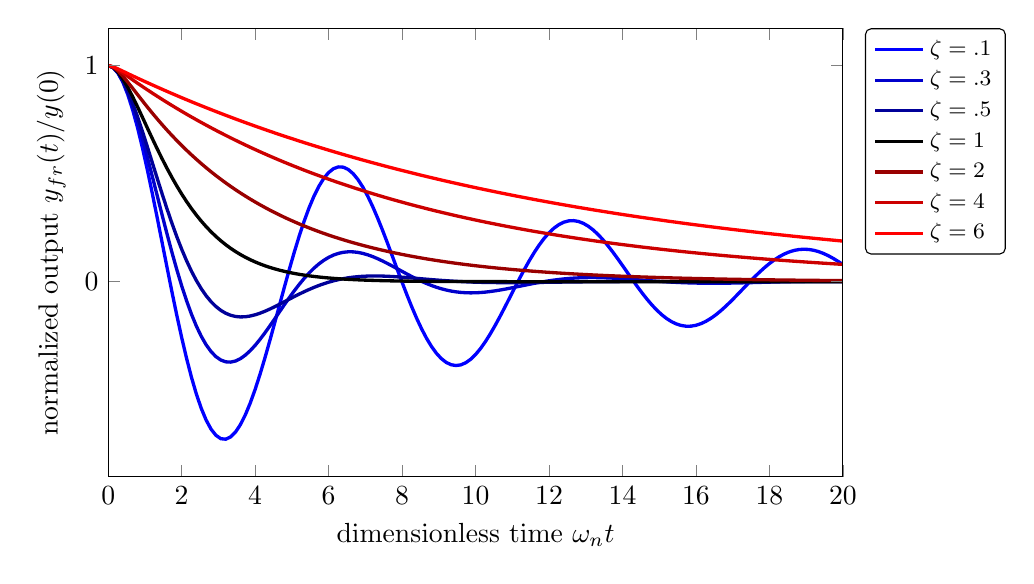
\begin{tikzpicture}
\newcommand{\ynot}{1.0}
\begin{axis}[
xlabel={dimensionless time $\omega_n t$},
ylabel={normalized output $y_\text{fr}(t)/y(0)$},
xmin=0, xmax=20,
% ymin=-15, ymax=10,
axis on top,
width=.9\linewidth,
height=.6\linewidth,
ytick={0,1},
tick pos=both,
tick label style={/pgf/number format/fixed},
scaled ticks=true,
legend style={
	legend pos=outer north east,
	cells={anchor=west},
	font=\footnotesize,
	rounded corners=2pt,
}
]
% \fill [gray!15] (rel axis cs:0,0) rectangle (rel axis cs:.675,1);
% \node at (rel axis cs:.275,.875) [anchor=south west] {transient};
% \node at (rel axis cs:.75,.875) [anchor=south west] {steady-state};
%
\newcommand{\z}{.1}
\addplot[
blue,
very thick,
domain=0:20,
samples=151,
] {\ynot*exp(-\z*x)/sqrt(1-\z^2)*cos(deg(sqrt(1-\z^2)*x)-atan(\z/sqrt(1-\z^2)))};
\addlegendentryexpanded{$\zeta = \z$}
%
\renewcommand{\z}{.3}
\addplot[
blue!80!black,
very thick,
domain=0:20,
samples=151,
] {\ynot*exp(-\z*x)/sqrt(1-\z^2)*cos(deg(sqrt(1-\z^2)*x)-atan(\z/sqrt(1-\z^2)))};
\addlegendentryexpanded{$\zeta = \z$}
%
\renewcommand{\z}{.5}
\addplot[
blue!60!black,
very thick,
domain=0:20,
samples=151,
] {\ynot*exp(-\z*x)/sqrt(1-\z^2)*cos(deg(sqrt(1-\z^2)*x)-atan(\z/sqrt(1-\z^2)))};
\addlegendentryexpanded{$\zeta = \z$}
%
\renewcommand{\z}{1}
\addplot[
black,
very thick,
domain=0:20,
samples=151,
] {\ynot*(1+x)*exp(-x)};
\addlegendentryexpanded{$\zeta = \z$}
%
\renewcommand{\z}{2}
\pgfmathsetmacro{\lone}{-\z+sqrt(\z^2-1)}
\pgfmathsetmacro{\ltwo}{-\z-sqrt(\z^2-1)}
\addplot[
red!60!black,
very thick,
domain=0:20,
samples=151,
] {
	\ynot*(
		\lone/(2*sqrt(\z^2-1))*exp(\ltwo*x) -
		\ltwo/(2*sqrt(\z^2-1))*exp(\lone*x)
	)
};
\addlegendentryexpanded{$\zeta = \z$}
%
\renewcommand{\z}{4}
\pgfmathsetmacro{\lone}{-\z+sqrt(\z^2-1)}
\pgfmathsetmacro{\ltwo}{-\z-sqrt(\z^2-1)}
\addplot[
red!80!black,
very thick,
domain=0:20,
samples=151,
] {
	\ynot*(
		\lone/(2*sqrt(\z^2-1))*exp(\ltwo*x) -
		\ltwo/(2*sqrt(\z^2-1))*exp(\lone*x)
	)
};
\addlegendentryexpanded{$\zeta = \z$}
%
\renewcommand{\z}{6}
\pgfmathsetmacro{\lone}{-\z+sqrt(\z^2-1)}
\pgfmathsetmacro{\ltwo}{-\z-sqrt(\z^2-1)}
\addplot[
red,
very thick,
domain=0:20,
samples=151,
] {
	\ynot*(
		\lone/(2*sqrt(\z^2-1))*exp(\ltwo*x) -
		\ltwo/(2*sqrt(\z^2-1))*exp(\lone*x)
	)
};
\addlegendentryexpanded{$\zeta = \z$}
%
\end{axis}
\end{tikzpicture}
\caption{free response $y_\text{fr}(t)$ of a second-order system with initial conditions $y(0)$ and $\dot{y}(0)=0$ for different values of $\zeta$. {\color{blue}Underdamped}, critically damped, and {\color{red}overdamped} cases are displayed.}
\label{fig:second_order_free_response}
\end{figure}

\subsection{Step response}
\tags{}

Second-order systems are subjected to a variety of forcing functions $f$.
In this lecture, we examine a common one: step forcing.
In what follows, we develop \keyword{forced response $y_\textnormal{fo}$} solutions.
\tags{}

Unit step forcing of the form $f(t) = u_s(t)$, where $u_s$ is the unit step function, models abrupt changes to the input.
The solution is found by applying zero initial conditions ($y(0) = 0$ and $\dot{y}(0) = 0$) to the general solution.
If the roots of the characteristic equation $\lambda_1$ and $\lambda_2$ are distinct, the forced response is
\tags{}
\begin{align}\label{eq:forced2}
	y_\text{fo}(t) = \dfrac{1}{\omega_n^2} 
	\left(
		1 -
		\dfrac{1}{\lambda_2-\lambda_1} 
		\left(
			\lambda_2 e^{\lambda_1 t} -
			\lambda_1 e^{\lambda_2 t}
		\right)
	\right)
\end{align}
where
\begin{equation} \label{eq:lambda3}
	\lambda_1 \text{, } \lambda_2 = -\zeta \omega_n \pm \omega_n \sqrt{\zeta^2 - 1}.
\end{equation}

Once again, there are five possibilities for the location of the roots of the characteristic equation $\lambda_1$ and $\lambda_2$, all determined by the value of $\zeta$.
However, there are three stable cases: underdamped, critically damped, and overdamped.
\tags{B, D}
\begin{description}
	\item[$\zeta\in(0,1)$ underdamped]
	In this case, the roots are distinct and complex: 
	\begin{equation}
		\lambda_1 \text{, } \lambda_2 = -\zeta \omega_n \pm j \omega_d.
	\end{equation}
	From \autoref{eq:forced2}, the forced step response is
	\begin{align}
		y_\textnormal{fo}(t) = 
		\dfrac{1}{\omega_n^2} 
		\left ( 
			1 - \dfrac{e^{-\zeta \omega_n t}}{\sqrt{1-\zeta^2}} 
			\cos(\omega_d t + \psi) 
		\right )
	\end{align}
	where the phase $\psi$ is
	\begin{equation}
		\psi =  -\arctan\dfrac{\zeta}{\sqrt{1-\zeta^2}}.
	\end{equation}
	This response overshoots, oscillates about, and decays to $1/\omega_n^2$.
	\item[$\zeta=1$ critically damped]
	The roots are equal and real:
	\begin{equation}
		\lambda_1 \text{, } \lambda_2 = -\omega_n
	\end{equation}
	so the forced step of \autoref{eq:forced2} must be modified; it reduces to
	\begin{align}
		y_\textnormal{fo}(t) = 
		\dfrac{1}{\omega_n^2} 
		\left ( 
			1 - e^{-\omega_n t} (1+\omega_n t)
		\right ).
	\end{align}
	This response neither oscillates nor overshoots its steady-state of $\dfrac{1}{\omega_n^2}$, but just barely.
	\item[$\zeta\in(1,\infty)$ overdamped]
	In this case, the roots are distinct and real, given by \autoref{eq:lambda3}.
	The forced step given by \autoref{eq:forced2} is the sum of two decaying real exponentials.
	These responses neither overshoot nor oscillate about their steady-state of $1/\omega_n^2$.
	With increasing $\zeta$, approach to steady-state slows.
\end{description}

\autoref{fig:second_order_step_response} displays the forced step response results.
These responses are inverted versions of the free responses of \autoref{lec:second_order_free_response}.
Note that a small damping ratio results in overshooting and oscillation about the steady-state value.
In contrast, large damping ratio results in neither overshoot nor oscillation.
However, both small and large damping ratios yield responses that take longer durations to approach equilibrium than damping ratios near unity.
For this reason, the damping ratio of a system should be close to $\zeta=1$.
There are tradeoffs on either side of one.
Slightly less yields faster responses that overshoot a small amount.
Slightly greater than one yields slower responses less prone to oscillation.
\tags{B, D}

\begin{figure}[bt]
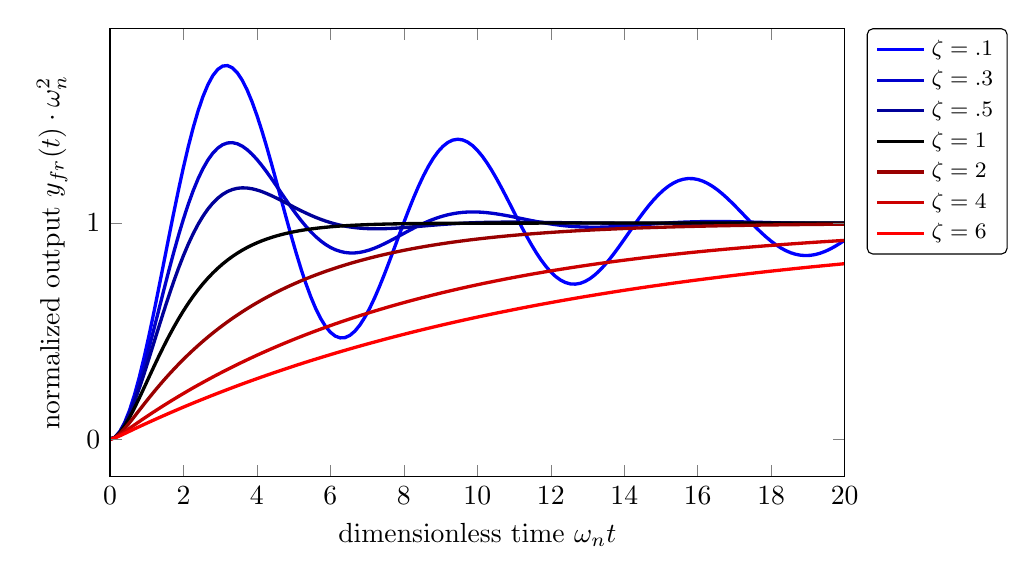
\begin{tikzpicture}
\begin{axis}[
xlabel={dimensionless time $\omega_n t$},
ylabel={normalized output $y_\text{fr}(t)\cdot\omega_n^2$},
xmin=0, xmax=20,
% ymin=-15, ymax=10,
axis on top,
width=.9\linewidth,
height=.6\linewidth,
ytick={0,1},
tick pos=both,
tick label style={/pgf/number format/fixed},
scaled ticks=true,
legend style={
	legend pos=outer north east,
	cells={anchor=west},
	font=\footnotesize,
	rounded corners=2pt,
}
]
% \fill [gray!15] (rel axis cs:0,0) rectangle (rel axis cs:.675,1);
% \node at (rel axis cs:.275,.875) [anchor=south west] {transient};
% \node at (rel axis cs:.75,.875) [anchor=south west] {steady-state};
%
\newcommand{\z}{.1}
\addplot[
blue,
very thick,
domain=0:20,
samples=151,
] {1-exp(-\z*x)/sqrt(1-\z^2)*cos(deg(sqrt(1-\z^2)*x)-atan(\z/sqrt(1-\z^2)))};
\addlegendentryexpanded{$\zeta = \z$}
%
\renewcommand{\z}{.3}
\addplot[
blue!80!black,
very thick,
domain=0:20,
samples=151,
] {1-exp(-\z*x)/sqrt(1-\z^2)*cos(deg(sqrt(1-\z^2)*x)-atan(\z/sqrt(1-\z^2)))};
\addlegendentryexpanded{$\zeta = \z$}
%
\renewcommand{\z}{.5}
\addplot[
blue!60!black,
very thick,
domain=0:20,
samples=151,
] {1-exp(-\z*x)/sqrt(1-\z^2)*cos(deg(sqrt(1-\z^2)*x)-atan(\z/sqrt(1-\z^2)))};
\addlegendentryexpanded{$\zeta = \z$}
%
\renewcommand{\z}{1}
\addplot[
black,
very thick,
domain=0:20,
samples=151,
] {1-(1+x)*exp(-x)};
\addlegendentryexpanded{$\zeta = \z$}
%
\renewcommand{\z}{2}
\pgfmathsetmacro{\lone}{-\z+sqrt(\z^2-1)}
\pgfmathsetmacro{\ltwo}{-\z-sqrt(\z^2-1)}
\addplot[
red!60!black,
very thick,
domain=0:20,
samples=151,
] {
	1 -
	1/(\ltwo-\lone)*
	(
		\ltwo*exp(\lone*x) -
		\lone*exp(\ltwo*x)
	)
};
\addlegendentryexpanded{$\zeta = \z$}
%
\renewcommand{\z}{4}
\pgfmathsetmacro{\lone}{-\z+sqrt(\z^2-1)}
\pgfmathsetmacro{\ltwo}{-\z-sqrt(\z^2-1)}
\addplot[
red!80!black,
very thick,
domain=0:20,
samples=151,
] {
	1 -
	1/(\ltwo-\lone)*
	(
		\ltwo*exp(\lone*x) -
		\lone*exp(\ltwo*x)
	)
};
\addlegendentryexpanded{$\zeta = \z$}
%
\renewcommand{\z}{6}
\pgfmathsetmacro{\lone}{-\z+sqrt(\z^2-1)}
\pgfmathsetmacro{\ltwo}{-\z-sqrt(\z^2-1)}
\addplot[
red,
very thick,
domain=0:20,
samples=151,
] {
	1 -
	1/(\ltwo-\lone)*
	(
		\ltwo*exp(\lone*x) -
		\lone*exp(\ltwo*x)
	)
};
\addlegendentryexpanded{$\zeta = \z$}
%
\end{axis}
\end{tikzpicture}
\caption{forced step response $y_\text{fo}(t)$ of a second-order system for different values of $\zeta$. {\color{blue}Underdamped}, critically damped, and {\color{red}overdamped} cases are displayed.}
\label{fig:second_order_step_response}
\end{figure}

\subsection{Impulse and ramp responses}

\begin{table}
\caption{responses of system $\dfrac{d^2 y}{dt^2} + 2 \zeta \omega_n \dfrac{d y}{dt} + \omega_n^2 y = f$ to different singularity forcing. Note that $\tau_1 = -1/\lambda_1$, $\tau_2 = 1/\lambda_2$, and $\psi = -\arctan(\zeta/\sqrt{1-\zeta^2})$.}
\begingroup
% \renewcommand*{\arraystretch}{2.5}
\def\mystrut{\rule[-2ex]{0ex}{6ex}}
\begin{adjustbox}{center}
\begin{tabular}{l l l}
	\toprule
	damping	& $f(t)$		& characteristic response \\ \midrule
	\mystrut $0 \le \zeta < 1$ & 
	$\delta(t)$	& 
	$\dfrac{e^{-\zeta \omega_n t}}{\omega_n \sqrt{1-\zeta^2}} \sin (\omega_d t)$ \\
	% \rule{0pt}{5ex} & 
	\mystrut &
	$u_s(t)$		& 
	$\dfrac{1}{\omega_n^2} \left ( 1 - \dfrac{e^{-\zeta \omega_n t}}{\sqrt{1-\zeta^2}} \cos (\omega_d t + \psi) \right ) $ \\
	\mystrut & 
	$u_r(t)$		
	& 
	$\begin{aligned} 
	\dfrac{1}{\omega_n^2} \left ( 
		t + \dfrac{e^{-\zeta \omega_n t}}{\omega_n} \left ( 
			\dfrac{}{} 2\zeta \cos \omega_d t + \dfrac{2\zeta^2 - 1}{\sqrt{1-\zeta^2}} \sin \omega_d t 
		\right ) - \dfrac{2 \zeta}{\omega_n} 
	\right )  
	\end{aligned}$ 
	\\
	\mystrut $\zeta = 1$	& $\delta(t)$	& $t e^{-\omega_n t}$  \\
	\mystrut & $u_s(t)$		& $\dfrac{1}{\omega_n^2} \left ( 1 - e^{-\omega_n t} - \omega_n t e^{-\omega_n t} \right )$ \\
	\mystrut & $u_r(t)$		& $\dfrac{1}{\omega_n^2} \left ( t + \dfrac{2}{\omega_n} e^{-\omega_n t} + t e^{-\omega_n t} - \dfrac{2}{\omega_n} \right )$ \\
	\mystrut $\zeta > 1$	& $\delta(t)$	& $\dfrac{1}{2 \omega_n \sqrt{\zeta^2 - 1}} \left ( e^{-t/\tau_1} - e^{-t/\tau_2} \right )$ \\
	\mystrut & $u_s(t)$		& $\dfrac{1}{\omega_n^2} \left ( 1 - \dfrac{\omega_n}{2 \sqrt{\zeta^2 - 1}} \left ( \tau_1 e^{-t/\tau_1} - \tau_2 e^{-t/\tau_2} \right ) \right )$ \\
	\mystrut &
	$u_r(t)$ & 
	$\begin{aligned} 
		\dfrac{1}{\omega_n^2} \left ( t - \dfrac{2 \zeta}{\omega_n}  + \dfrac{\omega_n}{2 \sqrt{\zeta^2 - 1}} \left ( \tau_1^2 e^{-t/\tau_1} - \tau_2^2 e^{-t/\tau_2} \right ) \right ) \nonumber 
	\end{aligned}$ 
	\\
	\bottomrule
\end{tabular}
\end{adjustbox}
\endgroup
\label{tab:forced_response_second_order}
\end{table}

The response to all three singularity inputs are included in \autoref{tab:forced_response_second_order}.
These can be combined with the free response of \autoref{eq:free1} using superposition.
\tags{}

\subsection{An example with superposition}
\tags{}

The results of the above are powerful not so much in themselves, but when they are wielded with the principle of superposition, as the following example shows.
\tags{}

\examplemaybe{
  MRFM cantilever beam with initial condition and forcing
  }{
  In magnetic resonance force microscopy (MRFM), the primary detector is a small cantilever beam with a magnetic tip.
  Model the beam as a spring-mass-damper system with mass $m=6$ pg,\footnote{One $\text{pg}=10^{-12}\text{g}=10^{-15}\text{kg}$.} spring constant $k = 15$ mN/m, and damping coefficient $B = 37.7\cdot10^{-15}$ N$\cdot$s/m. Magnetic input forces on the beam $u(t)$ are applied directly to the magnetic tip. That is, a Newtonian force-analysis yields the input-output ODE
  \begin{align*}
  	m \ddot{y} + B \dot{y} + k y = u,
  \end{align*}
  where $y$ models the motion of the tip.
  \begin{enumerate}
  	\item What is the natural frequency $\omega_n$?
  	\item What is the damping ratio $\zeta$?
  	\item Find the free response for initial conditions $y(0) = 10$ nm and $\dot{y}(0) = 0$.
  	\item Find the impulse (forced) response for input $u(t) = 3 \delta(t)$.
  	\item Find the total response for the initial condition and forcing, from above, are \emph{both} applied.
  \end{enumerate}
  }{
  \begin{enumerate}
  	\item 
	  Rewrite the differential equation in standard form:
	  \begin{align*}
	  	\ddot{y} + \dfrac{B}{m} \ddot{y} + \dfrac{k}{m} y &= \frac{1}{m} u \\
	  	\ddot{y} + 2\zeta\omega_n \ddot{y} + \omega_n^2 y &= \frac{1}{m} u
	  \end{align*}
	  Equate the coefficients:
	  \begin{align*}
	  	\dfrac{B}{m} = 2\zeta\omega_n 
	  	\quad \text{and} \quad
	  	\dfrac{k}{m} = \omega_n^2.
	  \end{align*}
	  Solving for $\omega_n$,
	  \begin{align*}
	  	\omega_n = \sqrt{\dfrac{k}{m}} = 62.8\text{ krad/s}.
	  \end{align*}
	  \item 
	  Solving for $\zeta$,
	  \begin{align*}
	  	\zeta &= \dfrac{B}{2\omega_n m} \\
	  	&= \dfrac{B}{2 m \sqrt{k}/\sqrt{m}} \\
	  	&= \dfrac{B}{2\sqrt{k m}} = 0.00005.
	  \end{align*}
	  This is very underdamped.
	  \item 
	  Superposition and tables. Don't forget about $1/m$.
	  \vspace{10\baselineskip}
  \end{enumerate}
}{%
ex:response_second_order%
}

\end{document}